\subsection{Controlled Evaluation on LoCoBench}
\label{sec:experiments}
\label{sec-experiments}
\label{sec-locobench}

\paragraph{Data.} LoCoBench \citep{anonlocobench} builds \emph{coherence ladders}: responses over
fixed claims that differ only in argument structure, with gold relation graphs. Each of its
\sThreeFamilies{} families is an expert answer written as a template with \emph{slots}; a slot
joins two claims, and its fillers draw no link, a support or a conflict between them. A ladder's
three rungs $\rho_0,\rho_1,\rho_2$ splice different fillers into the template, so they share every
other word, every claim and every verdict. Three ladder types are declared increasing: \cp{conflict}
removes conflicts between true claims, \cp{chain} adds entailments between them, and \cp{sign} goes
from deriving a false claim, through no link, to refuting it. Two are declared invariant: \cp{order}
permutes paragraphs and \cp{control} rewords one entailment. A three-vendor model committee reads
the gold relations pair by pair, and a ladder is admitted only if its gold graphs are ordered as
declared, by at least $0.05$ nats in $\Lambda$. The \sThreeLadders{} ladders have \sThreeItems{}
responses of 12--14 claims, two or three of them false; factuality labels give the verdict world and
stance the asserted world. Each ladder gives three rung pairs, so the \sThreeNConflict{} ladders of
each increasing type give $180$ pairs (App.~\ref{sec-full-locobench} and supplementary materials).

\paragraph{Setup.} The ladders induce \sThreeNIncPairs{} \emph{Increase} and \sThreeNInvPairs{}
\emph{Invariance} comparisons. Every score must rise on an Increase pair and stay equal on an
Invariance pair, up to a relative tie tolerance of $\sThreeRelTie$ (App.~\ref{app:setup-details}).
An \emph{arm} fixes the graph source: the \cp{gold} relations or one of four mining
configurations, each read at the verdict world (our default) and at the asserted world. On every
arm we also score $\LCS$'s three simplifications over the same graphs (\S\ref{sec:decomp}): the
signed weight sum $\Ssum$, the linear evidence $\Llin$ and the independent evidence $\Lambda^{\perp}$. Text baselines are length, DiscoScore (RC, LC, entity graph)
\citep{discoscore}, and judges using G-Eval \citep{geval} and a direct 1--5 rating of logical
coherence, averaged over five runs with GPT-6 and gpt-oss-120b; the judges see the response only.
Baselines that read only the claims tie on every pair (App.~\ref{app:results}). Error bars are 95\%
percentile-bootstrap intervals over families.

\begin{figure*}[t]
\centering
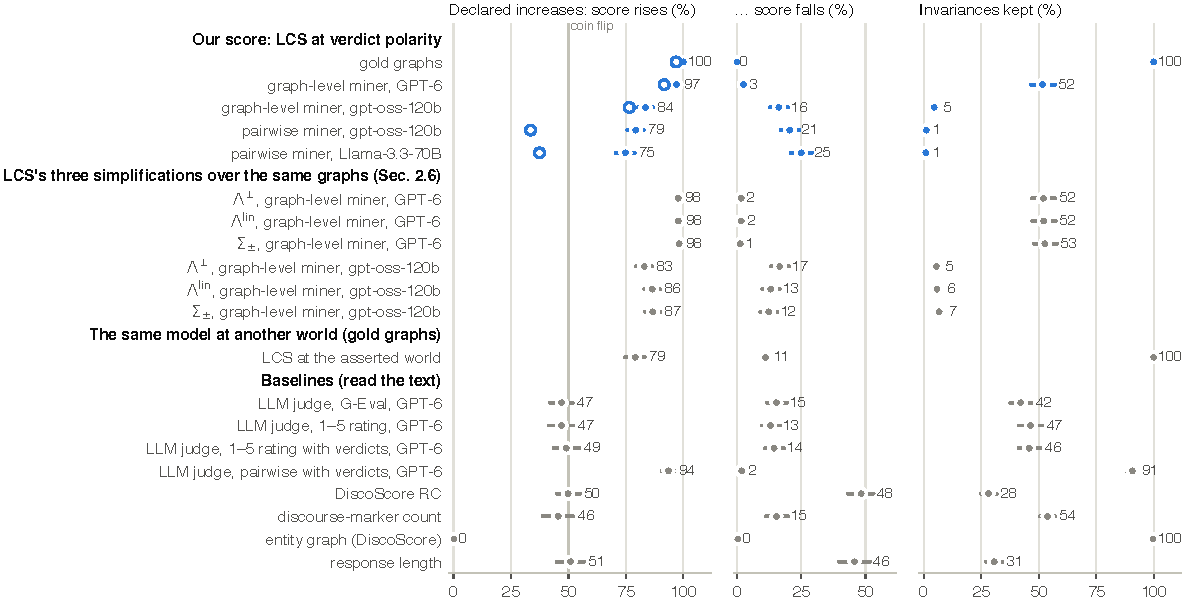
\includegraphics[width=1\textwidth]{figures/fig_ladders.pdf}
\caption{\textbf{Every score on LoCoBench's \sThreeNIncPairs{} declared increases and
\sThreeNInvPairs{} declared invariances.} \emph{Left:} share of Increase pairs on which the score
rises strictly; \emph{middle:} share on which it falls (the rest are ties). A score that ignores the
edits gets $0\%$ in both, a random one about $50\%$ in both. \emph{Right:} share of Invariance
pairs on which the score stays equal. \emph{Blue:}
$\LCS$ at the verdict world, on gold and mined graphs; hollow blue markers give the share that rises
by more than $\tau$. Judges average five runs, the verdict-aware
absolute judge three. \emph{Gray:} $\LCS$'s three simplifications over the graph-level arms'
graphs (all arms in Table~\ref{tab:signed}): the independent evidence $\Lambda^{\perp}$ (no
interaction), the linear evidence $\Llin$ (first order) and the signed weight sum $\Ssum$
(\S\ref{sec:decomp}); $\LCS$ at the asserted world; and the baselines. The entity graph reads the text but scores only nouns shared by nearby sentences, so it too
almost never moves.}
\label{fig:ladders}
\end{figure*}



\label{sec:exp-gold}
\label{sec:exp-mined}
\label{sec:exp-polarity}
\label{sec:exp-baselines}

\paragraph{Gold graphs check the implementation.} On gold graphs $\LCS$ satisfies all
\sThreeNIncPairs{} Increase and all \sThreeNInvPairs{} Invariance pairs (Figure~\ref{fig:ladders},
top row). This holds by construction, since the admission gate keeps only ladders whose gold
graphs are ordered, and it confirms that the implementation matches Theorem~\ref{thm:mono}.

\paragraph{The verdicts are needed.} At the \emph{asserted} world, which takes claims as the response
states them, gold graphs satisfy every \cp{conflict} and \cp{chain} pair but only
\sThreeGoldLamASign{} \cp{sign} pairs, as any signed score does: a derived falsehood counts as a
support there (App.~\ref{app:asserted-sign}).

\paragraph{Mined graphs: extraction sets the rate.} With mined graphs $\LCS$ rises on
\sThreeGraphGptLamIncPct\% (GPT-6 graph-level miner) to \sThreePairLlamaLamIncPct\% (pairwise Llama)
of the increases, and by more than $\tau=\sThreeTol$ on \sThreeGraphGptLamIncTolPct\% to
\sThreePairOssLamIncTolPct\%. Theorem~\ref{thm:mono} covers only pairs whose extracted graphs are
ordered as declared (\sThreeGraphGptDomForward{} of \sThreeNIncPairs{} with GPT-6, \sThreePairOssDomForward{}
with each pairwise miner), where $\LCS$ always rises (Figure~\ref{fig:dominance}). A weaker
graph-level miner from outside the committee's vendors (Llama-3.3-70B, \subLadders{} ladders) reaches
pair-level F1 \subLlamaPairF{} against \subGptPairF{} for GPT-6, and $\LCS$ rises on \subLlamaLcsInc\%
of its increases against \subGptLcsInc\%: results depend on the miner.

\begin{table}[t]
\centering\footnotesize
\setlength{\tabcolsep}{2.4pt}
\begin{tabularx}{\columnwidth}{@{}>{\raggedright\arraybackslash}Xcccc@{}}
\toprule
& $\Ssum$ & $\Llin$ & $\Lambda^{\perp}$ & $\LCS$ \\
\midrule
\multicolumn{5}{@{}l}{\emph{What each keeps} (\S\ref{sec:decomp})}\\
Violation outweighs support & -- & \checkmark & \checkmark & \checkmark \\
Curvature of $\lambda_r$ & -- & -- & \checkmark & \checkmark \\
Relations interact (A2) & -- & -- & -- & \checkmark \\
Range, unit & $\mathbb{R}$ & $\mathbb{R}$, nats & $\mathbb{R}$, nats & $(0,1)$, odds \\
\midrule
\multicolumn{5}{@{}l}{\emph{By construction} (\% of gold graphs; App.~\ref{app:results})}\\
Two halves score as the whole & \zsEqvSum & \zsEqvLin & \zsEqvIndep & \zsEqvLcs \\
Repetition counts less & \zsRepSum & \zsRepLin & \zsRepIndep & \zsRepLcs \\
Contested premise counts less & \zsDoubtSum & \zsDoubtLin & \zsDoubtIndep & \zsDoubtLcs \\
\midrule
\multicolumn{5}{@{}l}{\emph{LoCoBench increases satisfied} (\%)}\\
Gold graphs & \sThreeGoldWsumIncPct & \sThreeGoldLinIncPct & \sThreeGoldIndepIncPct & \sThreeGoldLamIncPct \\
Gold, 20\% of verdicts flipped & \vnWsumIncTwenty & \vnLinIncTwenty & \vnIndepIncTwenty & \vnLcsIncTwenty \\
GPT-6 graphs & \dcAttrWsum & \dcAttrLin & \dcAttrIndep & \dcAttrLcs \\
GPT-6, verifier's verdicts & \vfGptMinedWsumInc & \vfGptMinedLinInc & \vfGptMinedIndepInc & \vfGptMinedLcsInc \\
\midrule
\multicolumn{5}{@{}l}{\emph{ExpertQA} (\dcCountN{} answers, expert verdicts)}\\
$\rho$ with number of relations & $\dcCountWsumNrel$ & $\dcCountLinNrel$ & $\dcCountIndepNrel$ & $\dcCountLcsNrel$ \\
\bottomrule
\end{tabularx}
\caption{\textbf{$\LCS$ beside its three simplifications} (Prop.~\ref{prop:decomp}). Left to
right, each column adds one ingredient: the support/violation asymmetry ($\Llin$), the curvature of
the per-relation evidence $\lambda_r$ ($\Lambda^{\perp}=\sum_r\lambda_r$), and the interaction
$I_\R$ ($\LCS$). All four satisfy A1 and A3. The constructed edits hold or fail by definition; they
show what each score encodes, not how accurate it is (\zsEqvN{} gold graphs, \zsDoubtN{} for the
contested premise). Rows are read at the verdict world.}
\label{tab:three}
\end{table}

\paragraph{Where the four scores differ.} With correct verdicts all four satisfy every gold
increase (Table~\ref{tab:three}): each rung changes one relation's sign, which they read alike, and
the interaction is small on these graphs (median $|I_\R|=\dcIGoldAbsMedian$ nats against
$\dcLamGoldAbsMedian$ for $|\Lambda|$; Figure~\ref{fig:decomp}). Each step of the chain
$\Ssum\to\Llin\to\Lambda^{\perp}\to\LCS$ adds one ingredient, and the data separate them.
\begin{itemize}[leftmargin=1.2em,itemsep=1pt,topsep=2pt]
\item \textbf{The asymmetry decides the wrong-verdict case, and it is first order.} With 20\% of
  the verdicts flipped, $\Llin$, $\Lambda^{\perp}$ and $\LCS$ keep exactly the same increases (the
  curvature and interaction steps change none, \asapCI{\vnDiffILLoIncTwenty}{\vnDiffILHiIncTwenty}
  and \asapCI{\vnDiffLILoIncTwenty}{\vnDiffLIHiIncTwenty} points), and $\Llin$ beats $\Ssum$
  by\asapCI{\vnDiffLWLoIncTwenty}{\vnDiffLWHiIncTwenty} points. The gain is
  \asapCI{\vnDiffLWLoConflictTwenty}{\vnDiffLWHiConflictTwenty} on \cp{conflict} and a cost
  of\asapCI{\vnDiffLWLoChainTwenty}{\vnDiffLWHiChainTwenty} on \cp{chain}, so its net size depends
  on the mix of ladder types. With a closed-book GPT-6 verifier's verdicts on mined graphs, the four
  are within two points of one another (Table~\ref{tab:three}; $\LCS-\Ssum$
  in\asapCI{\vfGptMinedDiffloInc}{\vfGptMinedDiffhiInc}).
\item \textbf{On mined graphs no step helps.} On GPT-6 graphs $\LCS$ and $\Ssum$ disagree on
  \dcAttrDisagree{} of \dcAttrPairs{} increases. $\Ssum$ is right on \dcAttrSumWins{}, which turn
  at the asymmetry (\dcAttrSumWinsAsym), the curvature (\dcAttrSumWinsCurv) and the interaction
  (\dcAttrSumWinsInter) step; $\LCS$ is right on \dcAttrLcsWins. Exact McNemar tests of the three
  steps on the four mined arms (\mcFamily{} tests, Holm-adjusted; App.~\ref{app:decomp}) find no step
  at which the richer score is significantly better. The only step that survives the correction is a
  loss: on gpt-oss graphs the curvature costs (\mcCurvOssB{} pairs against \mcCurvOssC,
  $p=\mcCurvOssP$, Holm $\mcCurvOssHolm$), because a violated relation of high weight costs without
  bound. Nominally, on pairwise Llama the asymmetry helps (\mcAsymPairLlamaB{} against
  \mcAsymPairLlamaC, $p=\mcAsymPairLlamaP$) and the interaction costs (\mcInterPairLlamaB{} against
  \mcInterPairLlamaC, $p=\mcInterPairLlamaP$); neither survives.
\item \textbf{Three cases show the mechanisms} (App.~\ref{app:decomp}).
  \begin{itemize}[leftmargin=1.2em,itemsep=0pt,topsep=1pt]
  \item \emph{Asymmetry} (\dcExSumAsymLadder). The miner finds the added support (linear gain
    $\dcExSumAsymSupLin$ nats) and a spurious violated contradiction of weight
    \dcExSumAsymViolP{} ($-\dcExSumAsymViolLin$). $\Ssum$ rises and $\Llin$ falls, and so does $\LCS$
    (\dcExSumAsymLcsA{} to \dcExSumAsymLcsB).
  \item \emph{Interaction} (\dcExSumInterLadder). The rung's refutation of the falsehood cites a
    claim from which the response also draws an inference. The two overlap, so the refutation
    earns $\dcExSumInterDiscCtx$ nats in context against $\dcExSumInterDiscAlone$ alone; $\Lambda$
    moves by $\dcExSumInterDLam$ while $\Llin$ rises by $\dcExSumInterDLin$.
    This is the design consequence of \S\ref{sec:decomp}.
  \item \emph{The one pair $\LCS$ wins} (\dcExLcsCurvLadder). The miner trades three weak supports
    for two strong ones of the same total weight: $\Ssum$ moves by $\dcExLcsCurvDWsum$ and $\Llin$ by
    $\dcExLcsCurvDLin$; the curvature adds $\dcExLcsCurvDCurv$ nats, which decides the pair, and the
    interaction $\dcExLcsCurvDInter$, because the new supports link a chain.
  \end{itemize}
\item \textbf{On natural answers the weights keep $\LCS$ from counting relations, at the verdict
  world only.} Over \dcCountN{} ExpertQA answers \citep{expertqa} read at expert verdicts,
  the correlation with the number of mined relations falls along the chain: $\dcCountWsumNrel$,
  $\dcCountLinNrel$, $\dcCountIndepNrel$, $\dcCountLcsNrel$ ($\Ssum-\LCS$ in
  \asapCI{\dcCountDiffLo}{\dcCountDiffHi}). There $\LCS$ tracks the number of violated relations
  ($\rho=\dcCountLcsViol$). The value depends on the reading: at the asserted world $\LCS$
  correlates with the count at $\dcCountAssertedLcsNrel$, and with unsure claims counted true at
  $\dcCountUnsureTrueLcsNrel$ ($\Ssum$ $\dcCountUnsureTrueWsumNrel$). It describes the scores;
  whether counting relations is wrong is not something these data decide.
\end{itemize}

\paragraph{Text baselines and LLM judges.} Surface cues solve two of the three increasing types:
length rises on \sThreeBCtlLengthChain{} \cp{chain} pairs and a discourse-marker count on
\sThreeBCtlMarkersConflict{} \cp{conflict} pairs; only verdicts decide \cp{sign}. Judges rating one
response at a time do not separate \cp{chain} rungs: G-Eval with GPT-6 rises on
\sThreeBGevalGptChain{} pairs and falls on \sThreeBGevalGptChainFalls{} ($\LCS$:
\sThreeGraphGptLamChain), even given the claims, verdicts and our definition (rise\,/\,fall\,/\,tie
\fjAbsChainCounts). Asked which of two rungs is more coherent, in both orders and with the claims,
verdicts and definition, GPT-6 prefers the declared rung on \fjPairVIncRise\% of the increases and
calls \fjPairVInvTie\% of the invariance pairs equal: it comes close to $\LCS$ on increases
(difference\asapCI{\pcLcsPairVIncLo}{\pcLcsPairVIncHi} points) and keeps far more invariances
(\sThreeGraphGptLamInvPct\% for $\LCS$ exactly, \sThreeGraphGptLamInvTolPct\% within $\tau$;
\asapCI{\pcLcsPairVInvLo}{\pcLcsPairVInvHi}). $\LCS$ instead
scores each response on its own, with a guarantee and attribution, but rises on \nsLcsRise\% of
planted non-sequiturs, as on valid inferences, which the judge partly separates (App.~\ref{app:results}).
